%%%%%%%%Bilecik �eyh Edebali �niversitesi M�hendsilik Fak�ltesi%%%%
%%%%%%%%%%%Bilgisayar M�hendisli�i Proje I-II �al��mas�%%%%%%%%%%%%
%%%%%%%%%%%%%%%%%%%%%%LaTeX Class%%%%%%%%%%%%%%%%%%%%%%%%%%%%%%%%%%
\documentclass{BUP}
%%%%%%%%%%%%%%%%%%%%%%%%%%%%%%%%%%%%%%%%%%%%%%%%%%%%%%%%%%%%%%%%%%%%%%%%%%%
\begin{document}
\shorthandoff{=}%grafik komutlar�nda babelden kaynaklanan hatay� engeller.
%%%%%%%%%%%%%Proje I-II �al��malar�n�n B�l�mleri%%%%%%%%%%%%%%%%%%%%%%%%%%%
\thispagestyle{empty} %Bu sayfaya sayfa numaralar� yaz�lmaz
\begin{figure}[H]
\centering

\includegraphics[scale=0.2]{logomuz}
%Bu komutla resim dosyam�z� y�kl�yoruz.
\end{figure}
%sa�a 4 sol 2 a�a�� yukar� 3%
\begin{center}
\textbf{T.C.}\\
\textbf{B�LEC�K �EYH EDEBAL� �N�VERS�TES�}\\
\textbf{M�HEND�SL�K FAK�LTES�}

\textbf{B�LG�SAYAR M�HEND�SL��� B�L�M�}
\end{center}

\vspace*{4cm}%bir miktar bo�luk b�rakmak i�in
\begin{center}

\textbf{Tasar�m Projesi}\\
\textbf{�DEV-1}

\textbf{Ey�p �NDER}


\end{center}

\vspace*{\fill}
\begin{center}
\textbf{DANI�MANI:Uzman S�leyman UZUN}

\textbf{B�LEC�K}\\ 
\textbf{\today}
\end{center}

\thispagestyle{empty} %Bu sayfaya sayfa numaralar� yaz�lmaz

\begin{figure}[H]
\centering

\includegraphics[scale=0.2]{logomuz}
%Bu komutla resim dosyam�z� y�kl�yoruz.
\end{figure}
%sa� 4 sol 2 a�a�� yukar� 3%
\begin{center}
\textbf{T.C.}\\
\textbf{B�LEC�K �EYH EDEBAL� �N�VERS�TES�}\\
\textbf{M�HEND�SL�K FAK�LTES�}

\textbf{B�LG�SAYAR M�HEND�SL��� B�L�M�}
\end{center}

\vspace*{4cm}%bir miktar bo�luk b�rakmak i�in
\begin{center}
\textbf{BM308 Bilgisayar A�lar�}\\
\textbf{�DEV-1}

\textbf{Ey�p �NDER}


\end{center}

\vspace*{\fill}
\begin{center}
\textbf{ DANI�MANI:Uzman S�leyman UZUN}

\textbf{B�LEC�K}\\ 
\textbf{\today}
\end{center}

\pagenumbering{roman}%romen rakamlar� kullan�lmaya ba�lan�yor.
\setcounter{page}{2}% sayfa numaras�n� ii'den ba�lat�l�yor.
\centerline{\bf �ZET}
\addcontentsline{toc}{section}{�ZET}
\begin{center}
\textbf{Projenin Amac�}
\end{center} 
 \mbox{Bilgisayar A�lar�n�n ilk dersinde  g�rd���m�z konular�n peki�tirilmesi.}\\
 

\begin{center}
\textbf{Projenin Kapsam�}
\end{center}
 \mbox{�lk derste ��renilen kavramlar�n tan�mlar�n� yapmak , D�z ve Cross kablo ba�lant�s�n�}
 \mbox{ger�eklemek.}

\begin{center}
\textbf{Sonu�lar}
\end{center}
 \mbox{D�z ve Cross kablo  ba�lant�lar RJ-45 konnekt�r� ile yap�ld� ve derste ��renilen terimler}
 \mbox{peki�tirildi.}
%%%%%%%%%%%%%%%%%%%%%%%%%%%%%%%%%%%%%%%ABSTRACT%%%%%%%%%%%%%%%%%%%%%%%%%%%%%%%%%%%%%%%%%%
\newpage
\centerline{\bf ABSTRACT}
\addcontentsline{toc}{section}{ABSTRACT}
\begin{center}
\textbf{Project Objective}
\end{center}

 \mbox{}\dotfill\\
  \mbox{}\dotfill
%Bilecik �eyh Edebali University Department of Computer Engineering students is studied. The aim of project is work to create a template for writing \LaTeX\ writing the final report template in the Project, to be written.

\begin{center}
\textbf{Scope of Project}
\end{center}
 \mbox{}\dotfill\\
  \mbox{}\dotfill
%Bilecik �eyh Edebali University Computer Engineering Department Bilecik need to create a project template Latex codes assignment, involves the use of. The first part of the project consists of two parts, \LaTeX's development have been studied and why it is preferred that the use of information provided in the information. Faculty of Engineering of the university for the second part, Sheikh Edebali Bilecik Project Paper \LaTeX\ codes and are included.

\begin{center}
\textbf{Results}
\end{center}
 \mbox{}\dotfill\\
  \mbox{}\dotfill
%As a result, Bilecik Sheikh Edebali University Computer Engineering
%Department prepared a document that students can build project reports into \LaTeX. 
%include{4tesekkur}
\tableofcontents%bu komutun oldu�u yerde i�indekiler olu�turulur.
%\textbf{\centerline{\bf S�MGE L�STES�}}
\addcontentsline{toc}{section}{S�MGE L�STES�}

%\renewcommand*\listfigurename{\centerline{\bf\normalsize �EK�L L�STES�}}
\listoffigures%bu komutun oldu�u yerde �ekiller listesi olu�turulur
\addcontentsline{toc}{section}{�EK�L L�STES�}
%\renewcommand*\listtablename{\centerline{\bf\normalsize TABLO L�STES�}}
\listoftables%bu komutun oldu�u yerde tablolar listesi olu�turulur
\addcontentsline{toc}{section}{TABLO L�STES�}
\pagenumbering{arabic}%Sayfa numaralamas�n� arap rakamlar�yla yapar.
\setcounter{page}{1}%sayfa numaras�n� 1'den ba�lat�r.
\section{G�R��}    
\textbf{A� Nedir?} \\
Bilgisayarlar�n ve bilgisayarl� sistemlerin birbirleriyle  haberle�tikleri ,ileti�im kurduklar� ve kaynaklar�n� payla�t���  ortamd�r.\\
�leti�im ortamlar� Kablolu ve kablosuz ileti�im ortamlar� olarak ikiye ayr�l�r.\\ 
Kablolu ileti�im ortamlar�nda koaksiye(E� Eksenli)  ,�ift burgulu (Twisted-pair) ve fiber optik kablolar kullan�l�r.\\
\textbf{Koaksiyel (E� Eksenli) Kablo:}Anten veya uydu kablosunun daha ince olan�d�r.Bu kablolarla ba�lant� yapabiilmek i�in BNC konnekt�r kullan�lmal�d�r.\\
 \textbf{�ift Burgulu(Twisted -Pair)Kablo:}�ift Burgulu(Twisted -Pair) Kablo: UTP ve STP olmak �zere iki �e�idi bulunmaktad�r.�ift burgulu kablolarda genellikle UTP kablo tercih edilir STP  kablo daha maliyetlidir ve d��enmesi daha zordur.Bu kablo t�rlerinde bir a�da en fazla 100 m kablo olabilir.Bu t�r kablolarda -45 konnekt�r� ile ba�lant� sa�lan�r.D�z ve cross ba�lant� �ekillerinde ba�labilir d�z ba�lamada kablo renkleri kar��l�kl� olarak ayn� ba�lan�rken cross ba�lant�da 4 kablo sabit bulunmakta (-5-7-8 sabit) (1-3,3-1,2-6,6-2 ) numaral� kablolar ise �apraz ba�lan�r.Bu kablolama t�r�nde 10Base-T (10 Mbps),100Base-T (100 Mbps) ve1000Base-T (1000 Mbps) kablolama sistemleri kullan�labilir.10 Base-T:Saniyede maksimum 10 Mb aktar�m yapabilir.Sonundaki T kablonun t�r�n� belirtir(Twisted-Pair).\\
 \textbf{Fiber Optik Kablo:}Gelen elektrik sinyallerini ���k sinyaline �evirerek aktar�m sa�lar bu y�zden olduk�a h�zl� aktar�m g�c�ne sahiptir 70 km ye kadar iletim sa�layabilir.I���� cam t�p�n i�inde iletir.Maliyeti fazla olan bir kablolama t�r�d�r ve elektromanyetik alanlardan etkilenmez.�ok modlu , �ok modlu kademeli ve tek modlu �e�itleri bulunmaktad�r.\\
 \textbf{ A� Mimarileri ve Topolojileri }\\
A� mimarileri �stemci - Sunucu (Client - Server) Mimarisi ve t�rde�(Peer to peer) olmak �zere iki �e�ittir.\\
\textbf{ �stemci - Sunucu (Client - Server) :}Bu mimaride yaln�zca sunucu ve istemci bulunur sunucularda �zel i�letim sistemleri  bulunur. Her bilgisayar istemci veya sunucu olarak g�rev yapabilir istemciler kendi aralar�nda de�il yaln�zca  sunucularla haberle�irler.Her sunucu belirli bir i� �zerinde yo�unla�m��t�r.\\
\textbf{ T�rde�(Peer to peer):}Bilgisayarlar gem istemci hem sunucu olarak g�rev yapabilirler.Her bilgisayar e�ittir.On bilgisayardan fazla bilgisayarda performans d��er.\\
\textbf{ A� ��letim Sistemleri}\\
T�rde� Mimariler ��in;\\
Microsoft Windows for Workgroups vb\\
�stemci-sunucu / Sunucu Temelli\\
Linux\\
Unix\\
Windows NT 4.0, Windows Server 2000/2003\\
Novell Netware\\
\begin{center}
\textbf{ Co�rafi A��dan Bilgisayar A�lar�}
\end{center}


Bilgisayar a�lar� co�rafi yerle�imleri a��s�ndan �� temel gruba ayr�l�rlar.
\begin{itemize}
\item Yerel alan a�lar� (Local Area Network)\setstretch{0.1}
\item �ehirsel Alan A�lar� (Metropolitan Area Network\setstretch{0.1}
\item Geni� Alan A�lar� (Wide Area Network)
\end{itemize}
\textbf{ Yerel alan a�lar� (Local Area Network):}LAN, yerel a� ba�lant�s� (Local Area Network) anlam�na gelir. Ev, okul, k���k kurum ve kurulu�larda cihazlar�n ileti�imi ve kaynak payla��m� i�in olu�turulan a�d�r. Evlerimizde kulland���m�z bilgisayar a�lar� LAN t�r�ndedir. Yerel a� ba�lant�lar� olu�turulurken genellikle korumas� �ift burgulu kablo (UTP kablo) kullan�l�r.\\
\textbf{ �ehirsel Alan A�lar� (Metropolitan Area Network):}MAN, b�y�k i�yerlerinde ve �niversite kamp�slerinde kullan�lan a� t�r�d�r. �e�itli kaynaklarda kamp�s a�� olarak da adland�r�l�r. �lke geneline yay�lan i�letmelerin kendi aralar�nda olu�turduklar� a�lar da MAN t�r�nde ba�lant�d�r.\\
Geni� Alan A�lar� (Wide Area Network):WAN kapsad��� alan bak�m�ndan LAN ve  MAN dan b�y�kt�r. �ok �zak mesafedeki LAN  lar�n ba�lant�s� ile olu�turulur. WAN lar �zerinde on binlerce kullan�c� ve bilgisayar �al��abilir.\\ 
\begin{center}
\textbf{ A� Topolojileri}
\end{center}



\textbf{ Topoloji:}Bir a�da bilgisayarlar�n konumlar�n�, nas�l birbirine ba�lanaca��n� ve ne t�r bir veri ileti�imi i�inde olacaklar�n� belirleyen yap�ya denir.\\
\textbf{ Fiziksel topoloji:}A��n fiziksel olarak nas�l g�r�nece�ini belirler (Fiziksel katman).\\
\textbf{ Mant�ksal topoloji: }Bir a�daki veri ak���n�n nas�l olaca��n� belirler (Veri iletim katman�).\\

\begin{center}
\textbf{ A� Topoloji T�rleri}
\end{center}


\begin{itemize}
\item Do�rusal (Bus Topology)\setstretch{0.1}
\item Halka ( Token Ring Topology)\setstretch{0.1}
 \item Y�ld�z (Star Topology)\setstretch{0.1}
\item A�a�(Tree Topology)\setstretch{0.1}
\item Karma��k(Mesh Topology)
\end{itemize}
\textbf{ Do�rusal (Bus Topology)}Bu toplojide  bir kablo ortak yol olarak kullan�l�r ve bilgisayarlar bu kablo �zerine yerle�tirilir.Bu tek kabloya omurga denilebilir.Bu toplojide ula�t�r�lmak istenilen  sinyal yolun �zerinde do�rusal olarak dolan�r ve istasyonlar bu verinin kendisiyle ilgili olup olmad���na bakar kendiyle ilgiliyse  sinyali al�p gerekenleri yapar de�ilse sinyale m�dahele etmezler ve sinyal yoluna devam eder.


\textbf{Avantajlar�}\setstretch{0.1}
\begin{itemize}
\item A�a bir bilgisayar� ba�lamak olduk�a kolayd�r\setstretch{0.1}
\item Daha az uzunlukta kablo gerektirir.
\end{itemize}
\textbf{Dezavantajlar�}
\begin{itemize}
\item Sorun giderilmesi ve y�netimi zor olmas�.\setstretch{0.1}
\item K�s�tl� say�da istasyon ve k�sa mesafe kablo �zerinde olmas�.\setstretch{0.1}
\item Ana kabloda olu�an bir kopman�n t�m a��n �al��mas�n� engellemesi.\setstretch{0.1}
\item Eklenen her ilave istasyonun toplam a� performans�n� k�t� anlamda etkilemesi.\setstretch{0.1}
\item Omurga kablonun her iki ucunda sonland�r�c�lar�n bulunma zorunlulu�u.
\end{itemize}


\textbf{Halka ( Token Ring Topology):}
IBM taraf�ndan geli�tirilmi�tir.Her d���m kom�u iki d���me ba�l�d�r.�letim yolu halka bi�imindedir.Yolu kimin kullanaca��n� halka �zerindeki  dola�an  token(jeton)  karar verir.jetonu ele ge�iren d���m jetonu yoldan al�p verisini g�nderir verinin g�nderimi bitince jetonu yeniden yola koyar.UTP ve Stp kablo kullan�lmaktad�r.

\textbf{Avantajlar�}
\begin{itemize}
\item  �arp��ma olas�l��� d���kt�r.
\item T�m istasyonlar e�it eri�im hakk�na sahiptir.
\end{itemize}
\textbf{Dezavantajlar�}
\begin{itemize}
\item  Bir istasyonun ar�zas� durumunda t�m istasyonlar etkilenir.
\end{itemize}

\textbf{Y�ld�z (Star Topology):}Bu topolojide t�m d���mler ortak bir merkeze(hub veya switch) e ba�lan�r.Merkezdeki switch veya hub b�t�n veri ak���n� ve trafi�ini kontrol etmektedir. topolojiye yeni bir istasyon eklenmek istedi�inde ortak merkeze kablo vas�tas�yla kolay bir �ekilde ger�ekle�tirilir

\textbf{Avantajlar�}\setstretch{0.1}
\begin{itemize}
\item A�� kurmak kolayd�r\setstretch{0.1}
\item Bir bilgisayara ba�l� kablo\setstretch{0.1} bozuldu�unda a��n �al��mas� etkilenmez.
\item A�daki sorunlar� tespit etmek kolayd�r.
\end{itemize}

\textbf{Dezavantajlar�}\setstretch{0.1}
\begin{itemize}
\item Hub kullan�ld���nda a� trafi�i artar.\setstretch{0.1}
\item Do�rusala g�re daha fazla uzunlukta kablo gerektirir.\setstretch{0.1}
\item Hub veya Switch bozuldu�unda t�m a� �al��maz hale gelir.\setstretch{0.1}
\item Hub ve Switch gibi cihazlar nedeniyle do�rusala g�re kurulumu daha pahal�d�r.
\end{itemize}
\textbf{A�a�(Tree Topology):}Y�ld�z topolojisindeki a�lar� birbirine ba�lamak i�in kullan�l�r.Hiyerar�ik yap�daki a�lar i�in kullan�l�r.

\textbf{Avantajlar�}\setstretch{0.1}
\begin{itemize}
\item Her bir b�l�me (segment) ula�mak kolayd�r\setstretch{0.1}
\item Bir �ok �al��ma grubu bir araya getirilebilir. 
 \end{itemize}\newpage
\textbf{Dezavantajlar�}
\begin{itemize}
\item Her bir b�l�m�n uzunlu�u kullan�lan kablo ile s�n�rl�d�r.
\item Omurga kablosu bozuldu�unda b�l�mlerdeki a� trafi�i etkilenir.
\item Kurulumu ve d�zenlenmesi daha zordur.
\end{itemize}
\textbf{Karma��k(Mesh Topology)}
T�m d���mler a� i�erisinde birbirine ba�l�d�r.Daha �ok WAN da kullan�l�r. LAN da kullan�ld���nda t�m d���mlerin birbirine mutlaka ba�l� olmas� gerekmez.\\
\begin{center}
\textbf{A� Standartlar� ve Protokolleri}
\end{center}

\textbf{Ni�in A� Standartlar� �nemli?}
\begin{itemize}
\item Yeni ortaya ��kan sistemleri izlemek i�in.
\item Standartlar uluslararas� kapsamda olmal�.
\item  A��k sistemlerin temelini olu�turuyor.
\item Birlikte �al��maya olanak sa�l�yor.
\end{itemize}


\begin{center}
\textbf{OSI Katman Hizmetleri}
\end{center} 

\begin{center}
\begin{tabular}{|c|c|}\hline
Katman&G�revi\\
\hline
7.)Uygulama &Kullan�c� Uygulamalar�\\
\hline
6.)Sunum&Ayn� dilin konu�ulmas�; veri formatlama, �ifreleme\\
\hline
5.)Oturum&Ba�lant�n�n kurulmas� ve y�netilmesi\\
\hline
4.)Ta��ma &Verinin b�l�mlere ayr�larak kar�� tarafa gitmesinin kontrol edilmesi\\
\hline
3.)A�&Verinin b�l�mlere ayr�larak kar�� tarafa gitmesinin kontrol edilmesi\\
\hline
2.)Veri �letim&A� paketlerinin �er�evelere ayr�lmas�
\\
\hline
1.)Fiziksel& Fiziksel Veri Aktar�m�\\
\hline

\end{tabular}
\end{center}


\begin{center}
\begin{tabular}{|c|c|}\hline
Katman&PDU (Protocol Data Unit) Ad�i\\
\hline
7.)Uygulama &HTTP, FTP, SMTP\\
\hline
6.)Sunum&ASCII, JPEG, PGP\\
\hline
5.)Oturum&NetBIOS, DHCP\\
\hline
4.)Ta��ma &TCP, UDP, SPX\\
\hline
3.)A�&IP, IPX\\
\hline
2.)Veri �letim&Ethernet, Frame Relay, ISDN\\
\hline
1.)Fiziksel&Bit, Kablo, Konnekt�r\\
\hline

\end{tabular}
\end{center}



\begin{center}
\textbf{OSI de Verilerin Ad�}
\end{center}

\begin{center}
\begin{tabular}{|c|c|}\hline
Katman&Kullan�lan Veri Ad�\\
\hline
7.)Uygulama &Data(Veri)\\
\hline
6.)Sunum&Data\\
\hline
5.)Oturum&Data\\
\hline
4.)Ta��ma &Segment (B�l�m)\\
\hline
3.)A�&Segment(B�l�m)\\
\hline
2.)Veri �letim&Frame(�er�eve)\\
\hline
1.)Fiziksel&Bits (Bit)\\
\hline

\end{tabular}
\end{center}












\textbf{Ni�in Protokol Gerekli}

\textbf{Protokol:}�leti�im kurallar�n� temsil ederler.Ayg�tlar�n haberle�mesinde protokollere m�tab�k kal�n�p haberle�menin sa�lanmas� �nemlidir.
\begin{itemize}
\item Ortak bir �ekilde haberle�ebilmek anla�abilmek i�in\setstretch{0.1}
\item leti�im nas�l ba�lan�p nas�l sonlanaca��n� ve ne �ekilde devam edece�ini bilmek i�in.
\end{itemize}

\textbf{OSI:}Bilgisayar a�lar�n� tart��mak i�in yararl� bir modeldir.Her bir katman spesifik bir ileti�im sorununu belirler.\\
\textbf{TCP/IP:}Internet i�in bir protokol y���t�n�n kurulumu

\begin{center}

\textbf{A� Ba�lant� Ayg�tlar�}\\
\end{center}


\begin{center}

\textbf{OSI ve Cihazlar}\\

\end{center}

\begin{center}
\begin{tabular}{|c|c|}\hline
 OSI Katman�&Cihaz\\
\hline
7.)Uygulama &A� Ge�idi(Gateway)\\
\hline
6.)Sunum&A� Ge�idi(Gateway)\\
\hline
5.)Oturum&A� Ge�idi(Gateway)\\
\hline
4.)Ta��ma &A� Ge�idi(Gateway)\\
\hline
3.)A�&Y�nlendirici (Router)
Katman 3 Switch
\\
\hline
2.)Veri �letim&K�pr� (Bridge)
Katman 2 Switch
\\
\hline
1.)Fiziksel&NIC, Yineleyici (Repeater)
Hub, MAU
Kablo, Al�c� ve verici
\\
\hline

\end{tabular}
\end{center}


\textbf {Yineleyici(Repeater):}Kablonun kapasitesinden daha fazla  mesafelere ba�lant� sa�lamas� gerekti�inde sinyalin sinyalin y�kseltilmesini sa�layan cihazd�r.A� trafi�ini y�netmez sadece sinyali g��lendirir.OSI nin birinci katman�nda �al���r.

\textbf{Hub:}Birden fazla cihaz�n(Bilgisayar,yaz�c� kamera, tablet) birbiryle haberle�mesini sa�layan cihazd�r.Y�ld�z topolojide merkezde kullan�labilir. Switchlere g�re ak�ls�zd�rlar.

\textbf{Switch:}Ak�ll� Hub da denir.Gelen bilgisayar� sadece bilgisayarlara g�nderir.A� durumunu izler verinin g�nderip g�nderilmedi�ini test eder.

\textbf{K�pr�(Bridge):}OSI Veri �letim katman�nda �al���r.MAC adreslerini kullanarak paketleri iletir.K�pr�ler ba��ms�z �al��ma gruplar�n� birbirine ba�lamak i�in kullan�l�r. Birbiri ile ayn� topolojide veya farkl� topolojide olabilir. �rne�in bir y�ld�z ve bir halka topolojisinde a�lar�birbirine ba�layarak tek bir a� gibi g�sterir. Veri y�nlendirme i�lemi yapar. 
10 Mbps ve 100 Mbps a�lar� birbirine ba�layabilir 


\textbf{Router(Y�nlendirici):}A�lar aras� (LAN-LAN, LAN-WAN, WAN-WAN) haberle�menin yap�labilmesi i�in ara ba�lant�y� sa�lar. 


\textbf{Gateway(A� Ge�idi):}Ge�it, iki farkl� protokol aras�ndaki d�n���mleri sa�lar. Bu cihaz bir K�pr�, Switch veya Y�nlendirici olabilir.Genellikle Y�nlendirici (Router) bu g�revi �stlendi�inden varsay�lan a� ge�idi (default gateway) olarak o tan�ml�d�r.\newpage

\begin{center}
\textbf{D�z ve Cross Kablo Yap�m� Hakk�nda}
\end{center}

2 metre UTP kabloyu 2 ye b�l�p birer metrelik  iki kablo elde ettim D�z ba�lant� i�in �ekil 1 de g�r�len �ekilde kablolar� renklerine g�re dizdim.Dizdikten sonra Bunlar� RJ-45 konnekt�r�ne sokup s�k��t�c� ile konnekt�re bast�r�p kabloyu konnekt�re sabitledim kablonun di�er ucu i�inde ayn� i�lemi tekrarlad�m.



\begin{figure}[H]
\begin{center}
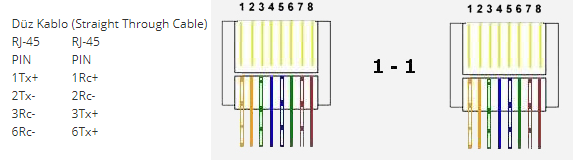
\includegraphics[]{a.png}
\caption{D�z Kablo Ba�lant�s�}
\end{center}
\end{figure}


Di�er 1 metrelik kabloylada Cross ba�lant� yapt�m.A�a��da �ekil 2 de g�r�len �eklin solundaki kablo renk dizlimlerini dizip RJ-45 konnekt�r�ne oturtup s�k��t�r�c� ile konnekt�r� s�k��t�r�p kabloya oturttum.Di�er taraf� i�in �ekil 2  nin  sa� taraf�ndaki renk dizilimlerini dizip konnekt�re yerle�tirip s�k��t�r�c� ile s�k��t�rd�m.B�ylelikle Cross kablo elde etmi� oldum. \\

\begin{figure}[H]
\begin{center}
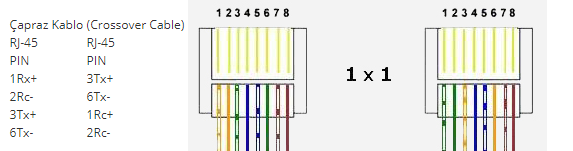
\includegraphics[]{b.png}
\caption{Cross Kablo Ba�lant�s�}
\end{center}
\end{figure}

Son olarak kablolar�n sa�laml���n� test etmek i�in  Ledli Kontrol Ba�lant� Cihaz� ile kablolar� test ettim d�z kabloda kar��l�kl� ledler yanarken Cross kabloda ise  kar��l�kl� ���klar�n yanmad��� 1 ile 3 �n 3 ile 1 in 2 ile 6 n�n 6 ile 2 nin �apraz olarak yand���n� g�rd�m geriye kalan kablo numaralar�n�n kar��l�kl� olarak ledleri yand�.


Kontrol Ba�lant� Cihaz� (Ledli) a�a��da �ekil 3 te  verilmi�tir.


\begin{figure}[H]
\begin{center}
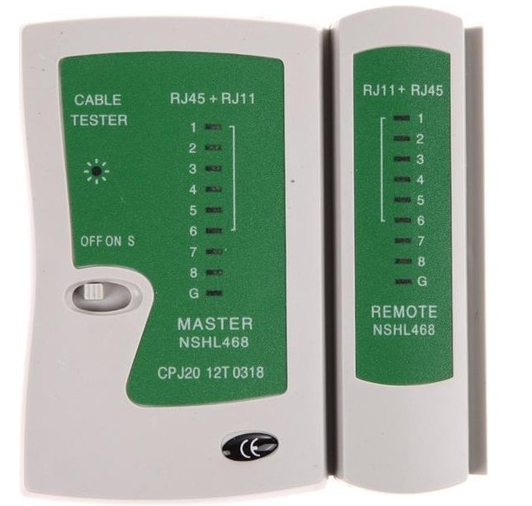
\includegraphics[]{c.png}
\caption{Network Kablo Test Cihaz�}
\end{center}
\end{figure}


%\section{}

%\section{}

%\section{SONU�LAR VE �NER�LER}

%\section{EKLER}

%\renewcommand{\refname}{KAYNAKLAR}
\addcontentsline{toc}{section}{KAYNAKLAR}
\begin{thebibliography}{99}%kaynak ortam� olu�turmak i�in
%%%%Kaynak Web sayfas�ndan al�nm�� ise%%%%%%%%%%%%%%%%%
\bibitem{k:1} CTAN,\url{http://zelmanov.ptep-online.com/ctan/lshort_turkish.pdf} [Ziyaret Tarihi: 4 Kas�m 2011]\textcolor{red}{---> Kaynak yazar� bilinmeyen yabanc� bir �al��madan al�nm�� ise: }
\bibitem{k:2} Anonymous, 1989, Farm accountancy data network, an
A-Z of methodology, Commission Report of the EC, Brussels, 16-19. 
\bibitem{k:3} \url{http://akgul.bilkent.edu.tr/Yunus/lshort.pdf}
\textcolor{red}{---> Kaynak kongreden al�nm�� ise:}
\bibitem{k:4} Calvalho, M. ve Ludermir, T.B., 2007, Particle Swarm Optimization of Neural Network Architectures and Weights, Seventh International Conference on Hybrid Intelligent Systems, Almanya, 336-339. 
\textcolor{red}{---> Kaynak akt�el dergi ve gazete haberinden al�nm�� ise:} 
\bibitem{k:5} �evkli, M., ve Yenisey, M. M., 2006, At�lye Tipi 
�izelgeleme Problemleri i�in Par�ac�k S�r� Optimizasyonu Y�ntemi, �t�dergisi/d M�hendislik, Cilt 5, Say� 2(1), 58-68.
\textcolor{red}{---> Kaynak akt�el dergi ve gazete haberinden al�nm�� ise:}
\bibitem{k:6} \url{http://kisi.deu.edu.tr/umit.akinci/latexseminer.pdf}\textcolor{red}{---> Kaynak yazar� bilinmeyen ulusal bir �al��madan al�nm�� ise:}
\bibitem{k:7} Anonim, 2006, Tar�m istatistikleri �zeti, D�E Yay�nlar�, No;12, Ankara, 22-23. 
\textcolor{red}{---> Kaynak yazar� bilinmeyen ulusal bir �al��madan al�nm�� ise:}
\end{thebibliography}
%\centerline{\textbf{�ZGE�M��}}
\addcontentsline{toc}{section}{�ZGE�M��}
\begin{table}[H]
{
\renewcommand{\arraystretch}{1.5}
\begin{tabular}{l@{\bf :}l}
\multicolumn{2}{l}{\underline{\bf K���SEL B�LG�LER}}\cr
\textbf{Ad� Soyad�}& Ey�p �nder    \cr
\textbf{Uyru�u}& TC\;  \cr
\textbf{Do�um Yeri ve Tarihi}& K���K�EKMECE 1996 \;     \cr
\textbf{Adres}&\; Ertu�rulgazi Mahallesi Stadyum Sokak No:45 Bilecik/Merkez      \cr
\multicolumn{1}{l}{}&      \cr
\textbf{Telefon}&\; 05437632767     \cr
\textbf{e-mail}&\; eyponderll@gmail.com   \cr
\multicolumn{1}{l}{}&\cr
\multicolumn{2}{l}{\underline{\bf E��T�M DURUMU}}\cr
\textbf{Lisans ��renimi}&\; B�E� Bilgisayar M�hendisli�i B�l�m�\cr
\textbf{Bitirme Y�l�}&\;    \cr
\textbf{Lise}& \;    \cr
\multicolumn{1}{l}{}&\cr
\multicolumn{2}{l}{\underline{\bf �� DENEY�MLER�}}\cr
\textbf{Y�l}&\;     \cr
\textbf{Kurum}& \;    \cr
\textbf{Stajlar}&\;     \cr
\multicolumn{1}{l}{}&\cr
\multicolumn{2}{l}{\underline{\bf �LG� ALANLARI:}}\cr
\multicolumn{1}{l}{}&\cr
\multicolumn{2}{l}{\underline{\bf YABANCI D�LLER:}}\cr
\multicolumn{1}{l}{}&\cr
\multicolumn{2}{l}{\underline{\bf BEL�RTMEK �STED���N�Z D��ER �ZELL�KLER:}}
\end{tabular}}
\end{table}
\shorthandon{=}
\end{document}
%%%%%%%%%%%%%%%%%%%%%%%%%%%B�TT�%%%%%%%%%%%%%%%%%%%%%%%%%%%%%%%%%%%%%%%%%%%%%
